%%%%%%%%%%%%%%%%%%%%% chapter.tex %%%%%%%%%%%%%%%%%%%%%%%%%%%%%%%%%
%
% Capítulo Algoritmos Sequenciais
%
% Laboratório 1: Sequência de LEDs
%
%%%%%%%%%%%%%%%%%%%%%%%% Springer-Verlag %%%%%%%%%%%%%%%%%%%%%%%%%%
\chapter{Algoritmos Sequenciais}
\label{intro} % Always give a unique label
% use \chaptermark{}
% to alter or adjust the chapter heading in the running head

\abstract{O objetivo deste capítulo é apresentar uma prática de laboratório que utiliza um algoritmo sequencial para acender três LEDs sequencialmente utilizando a placa Intel Galileo.}

\begin{figure}[h]
\centering
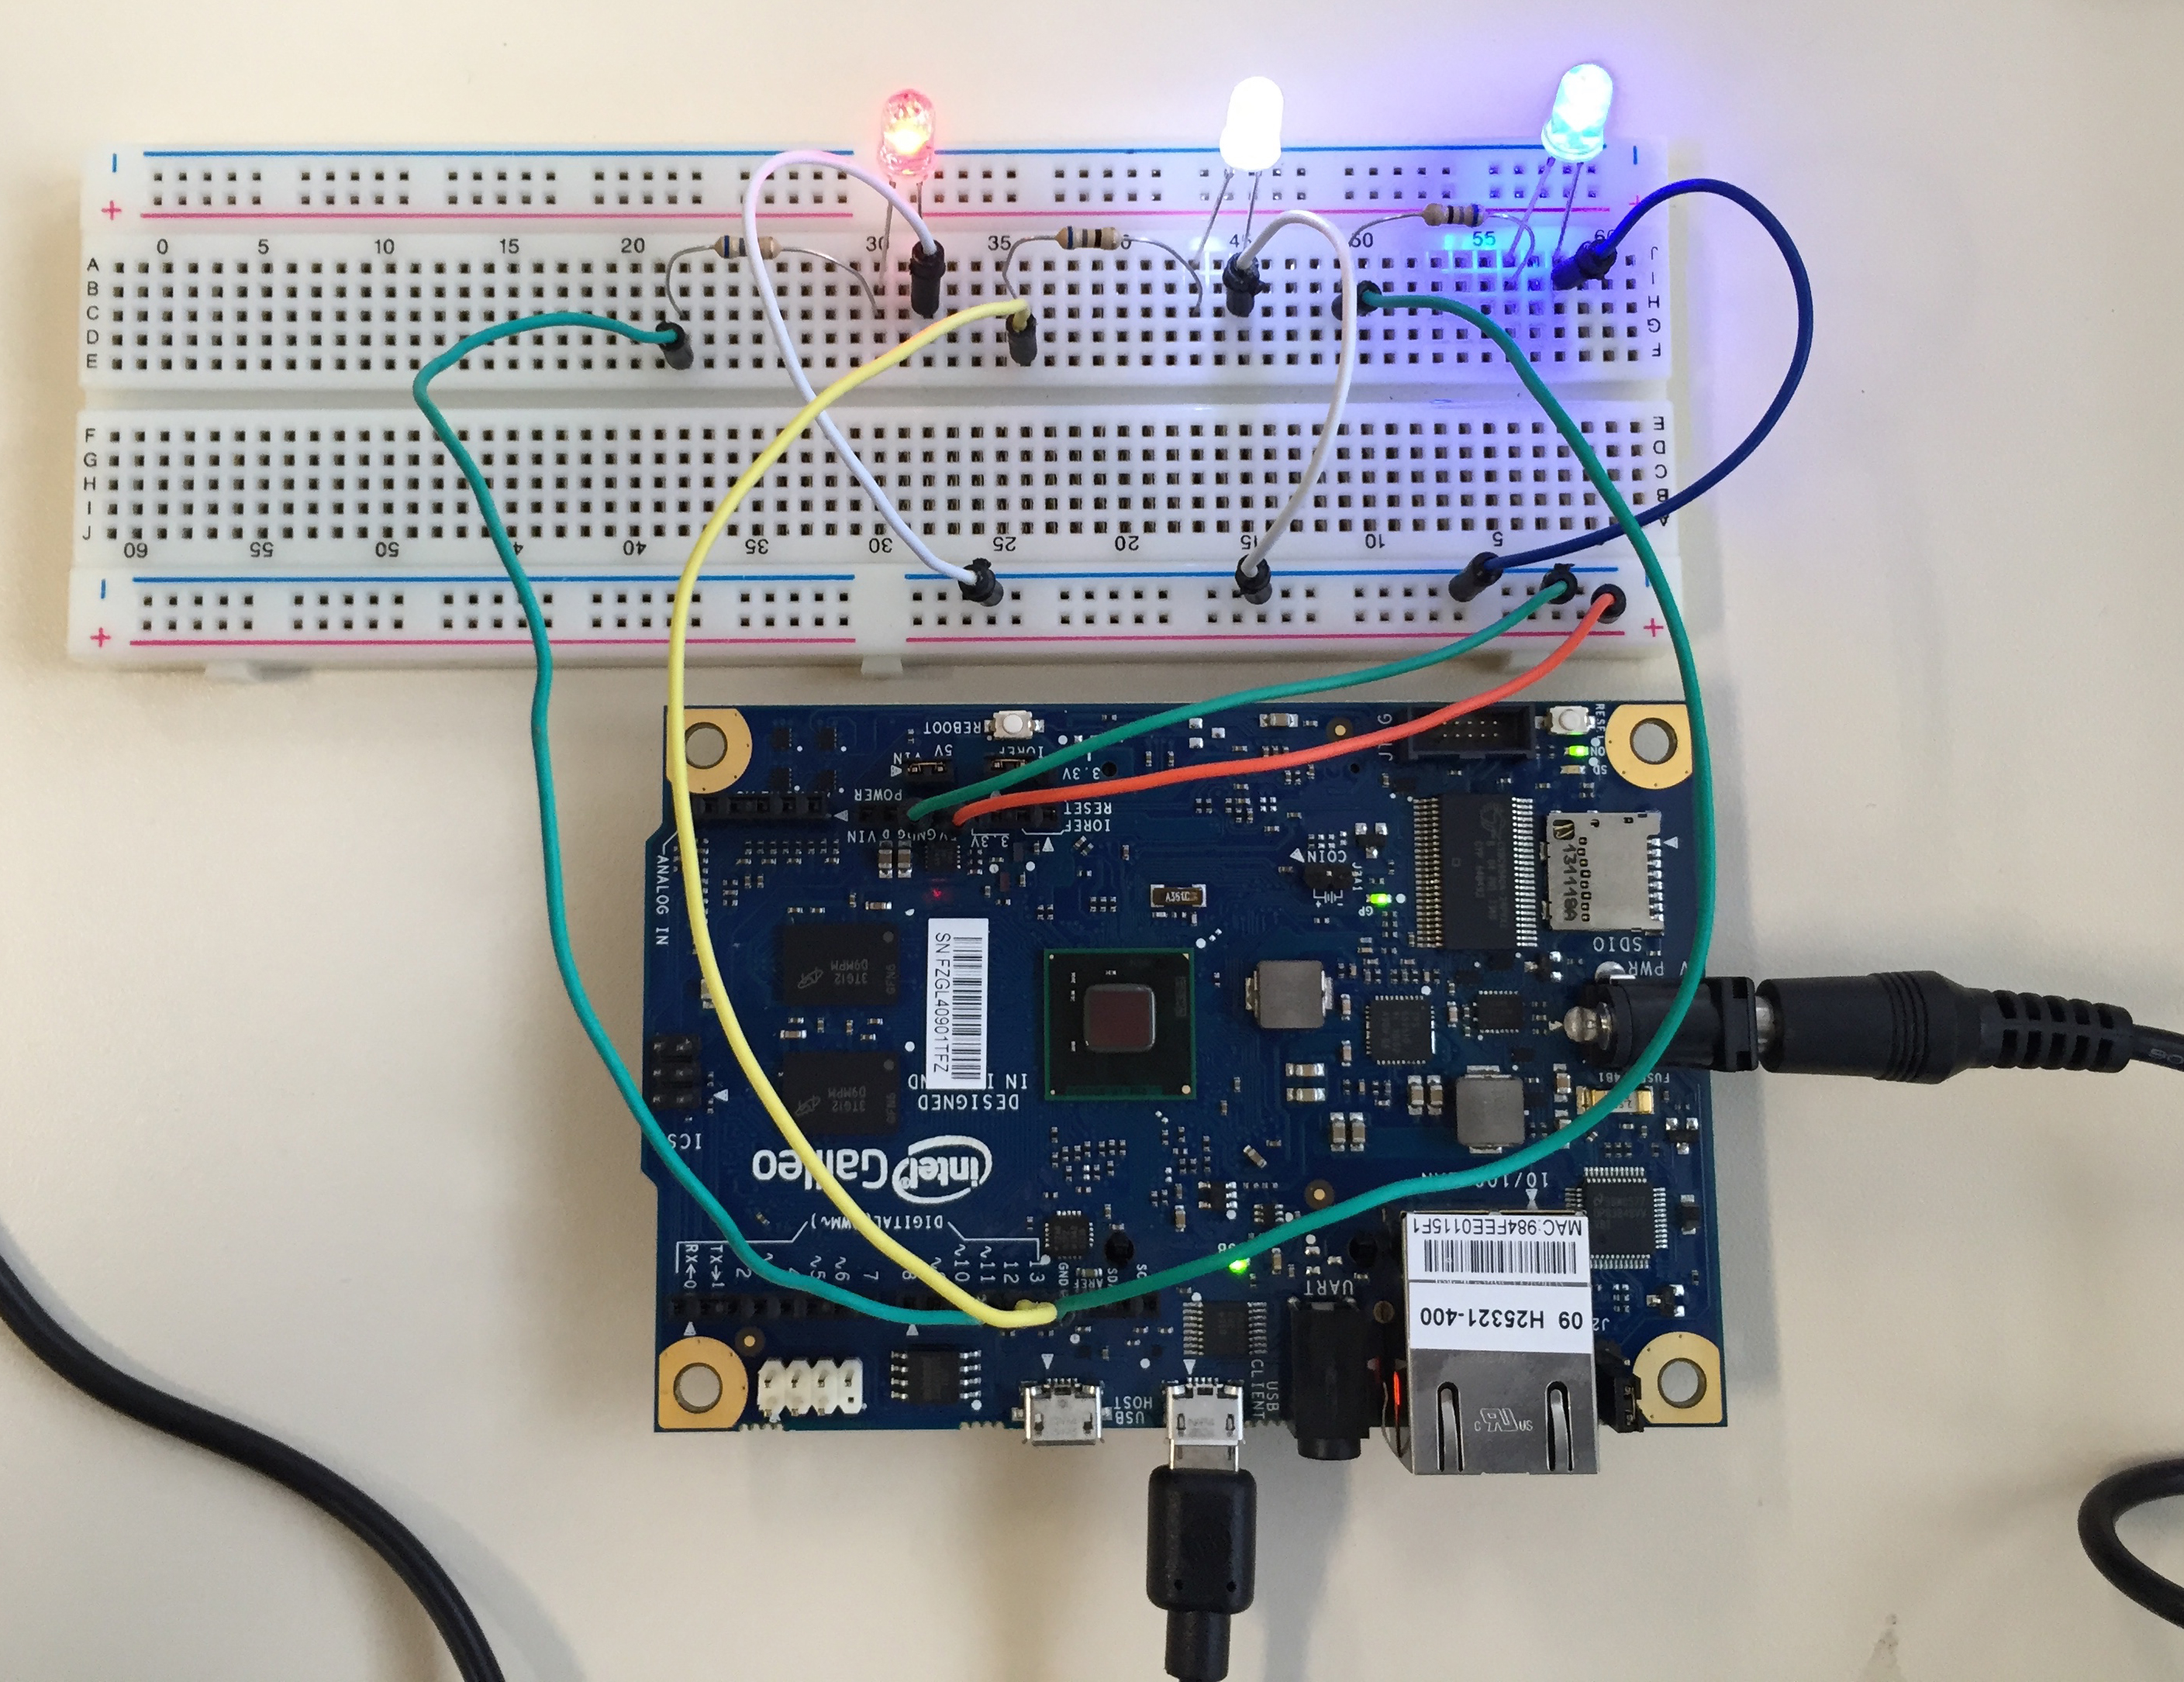
\includegraphics[scale=0.12]{chapter2/real.jpg}
\caption{Sequência de LEDs}
\label{fig:1}
\end{figure}

\section{Componentes necessários}
\label{sec:1}

Para o desenvolvimento da prática serão necessários além da placa Intel Arduino e da protoboard, três LEDs que podem ser de cores diferentes, três resistores de 68$\Omega$ e fios para as conexões.
Observação: para evitar possíveis danos aos componentes da placa, recomenda-se ligar a mesma a fonte primeiro e depois ao usb do computador. 

\section{Diagrama}
\label{sec:2}

As conexões entre a placa, a protoboard e os componentes deverão ser feitas seguindo o diagrama (Figura 2.2) abaixo:

\begin{figure}[h]
\centering
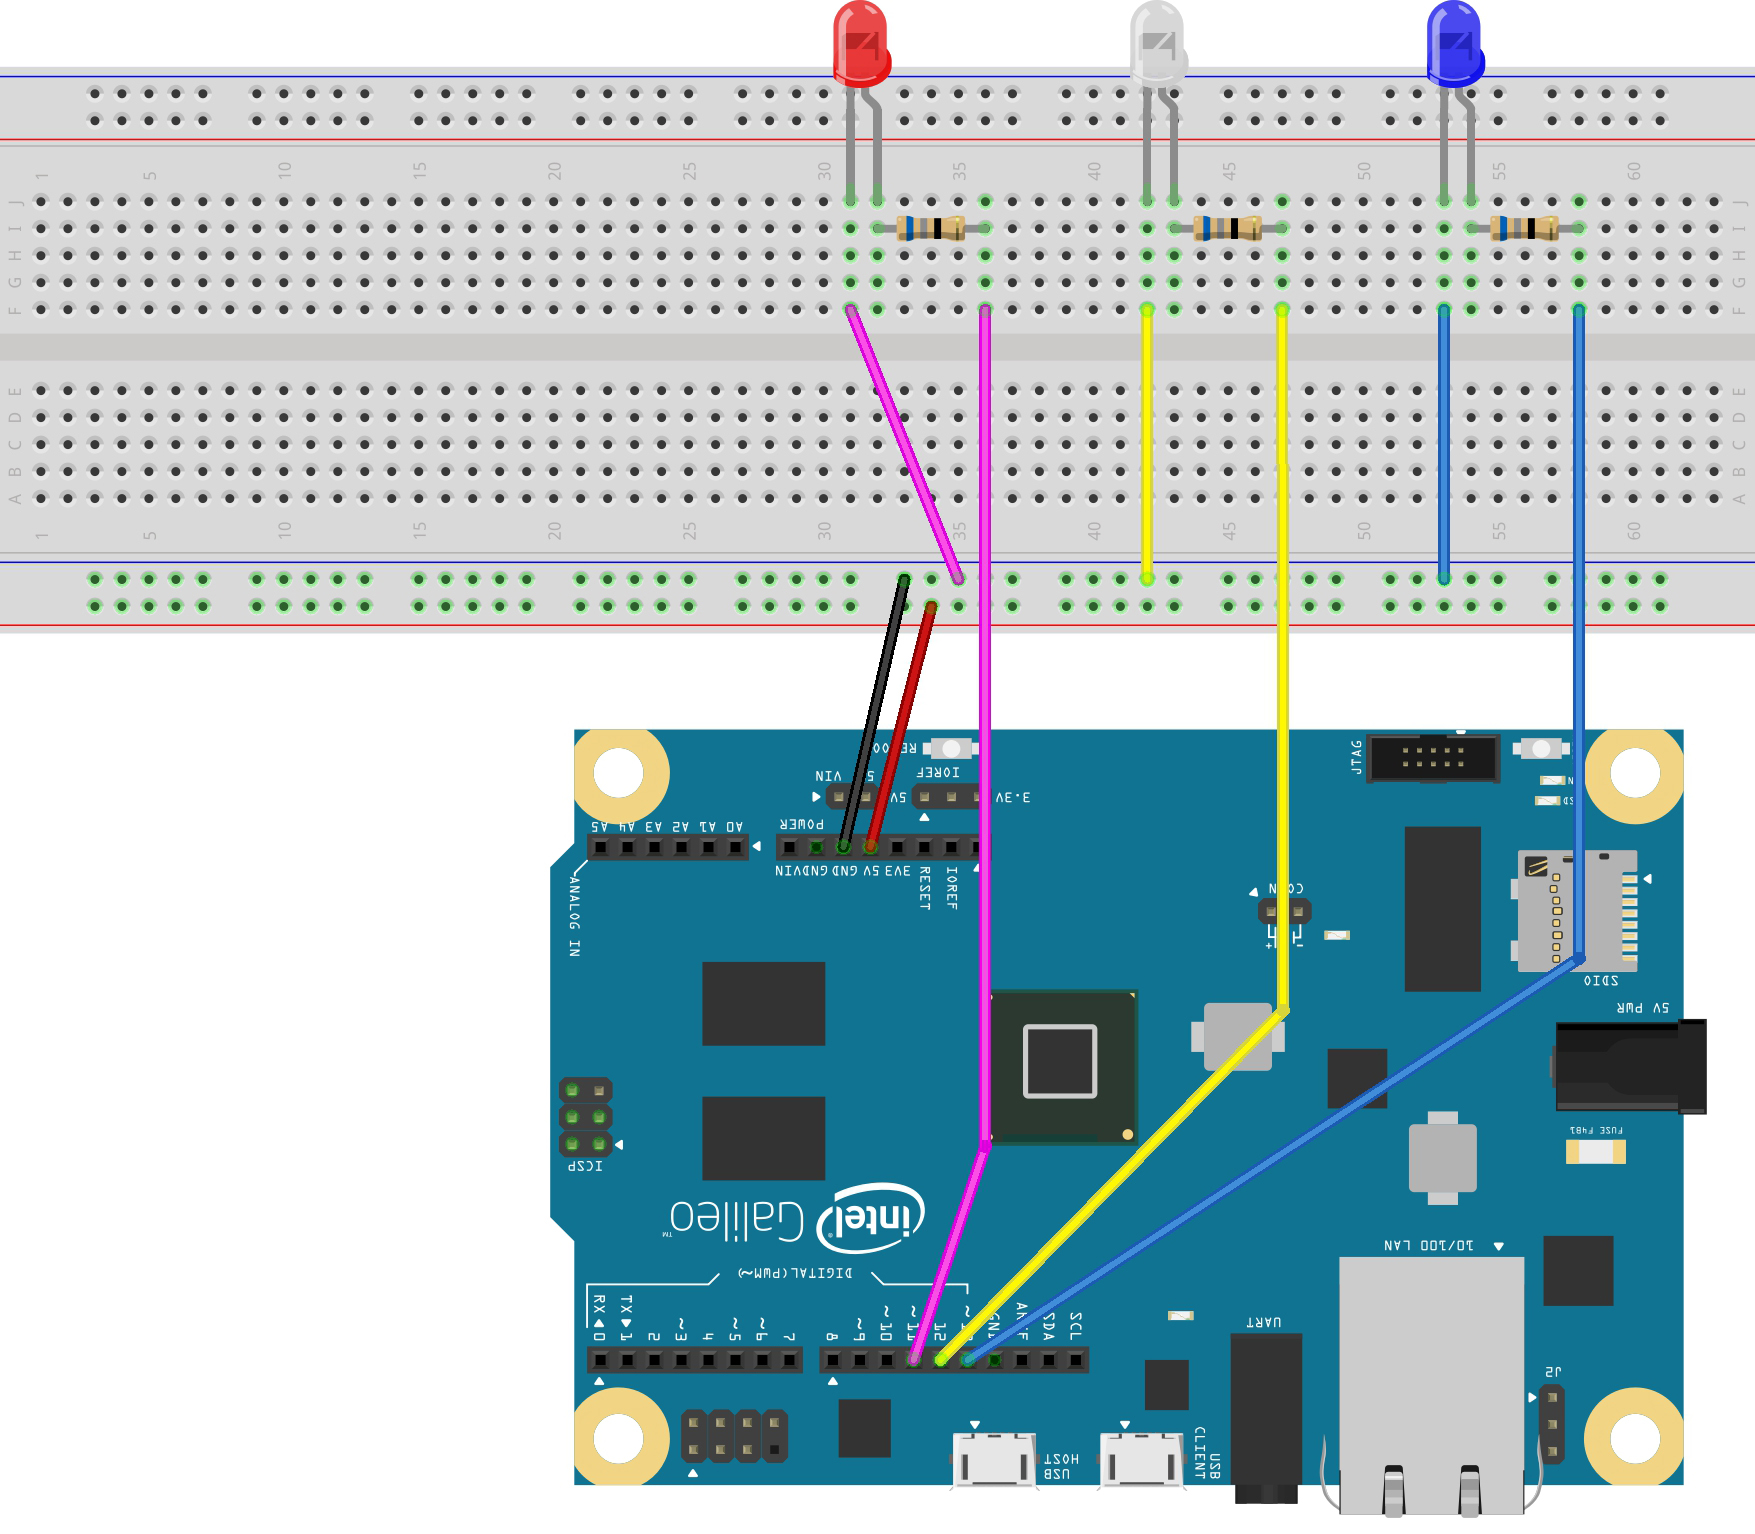
\includegraphics[scale=0.8]{chapter2/algseq.jpg}
\caption{Laboratório 1}
\label{fig:2}
\end{figure}


\section{Código-fonte}
\label{sec:3}
Através da IDE Arduino, o código (algoritseq.ino) abaixo é compilado e tranferido para a placa.

\lstinputlisting[float=h]{chapter2/algoritseq.ino}

Como pode-se observar no código acima, as linhas \textbf{int ledPin1 = 13;}, \textbf{int ledPin1 = 12;} e \textbf{int ledPin1 = 11;} identificam os pinos para cada LED, as linhas \textbf{pinMode(ledPin1, OUTPUT);}, \textbf{pinMode(ledPin2, OUTPUT);} e \textbf{pinMode(ledPin3, OUTPUT);} configuram os pinos 13, 12 e 11 da placa, que estão um a um conectados aos resistores e aos LEDs, como saídas, as linhas \textbf{digitalWrite(ledPin1, HIGH);}, \textbf{digitalWrite(ledPin2, HIGH);} e \textbf{digitalWrite(ledPin3, HIGH);} acendem os LEDs, as linhas \textbf{digitalWrite(ledPin1, LOW);}, \textbf{digitalWrite(ledPin2, LOW);} e \textbf{digitalWrite(ledPin3, LOW);} apagam os LEDs e as linhas \textbf{delay(250);} e \textbf{delay(500);} fazem o programa esperar por 500ms e por 250ms respectivamente. Como pode-se observar, por se tratar de um algoritmo sequencial, os eventos ocorrem na ordem em que estão escritos no código, porém por causa da natureza repetitiva da rotina loop() a mesma sequencia de eventos se repete até que a placa seja desligada ou que um outro programa seja transferido para a mesma.

\section{Conclusão}
\label{sec:4}
Nesta prática foi possível observar como ser comportam os algoritmos sequenciais na placa Intel Galileo e construir um circuito capaz de acender três LEDs sequencialmente (Figuras 2.3, 2.4, 2.5, 2.6).

\begin{figure}[h]
\centering
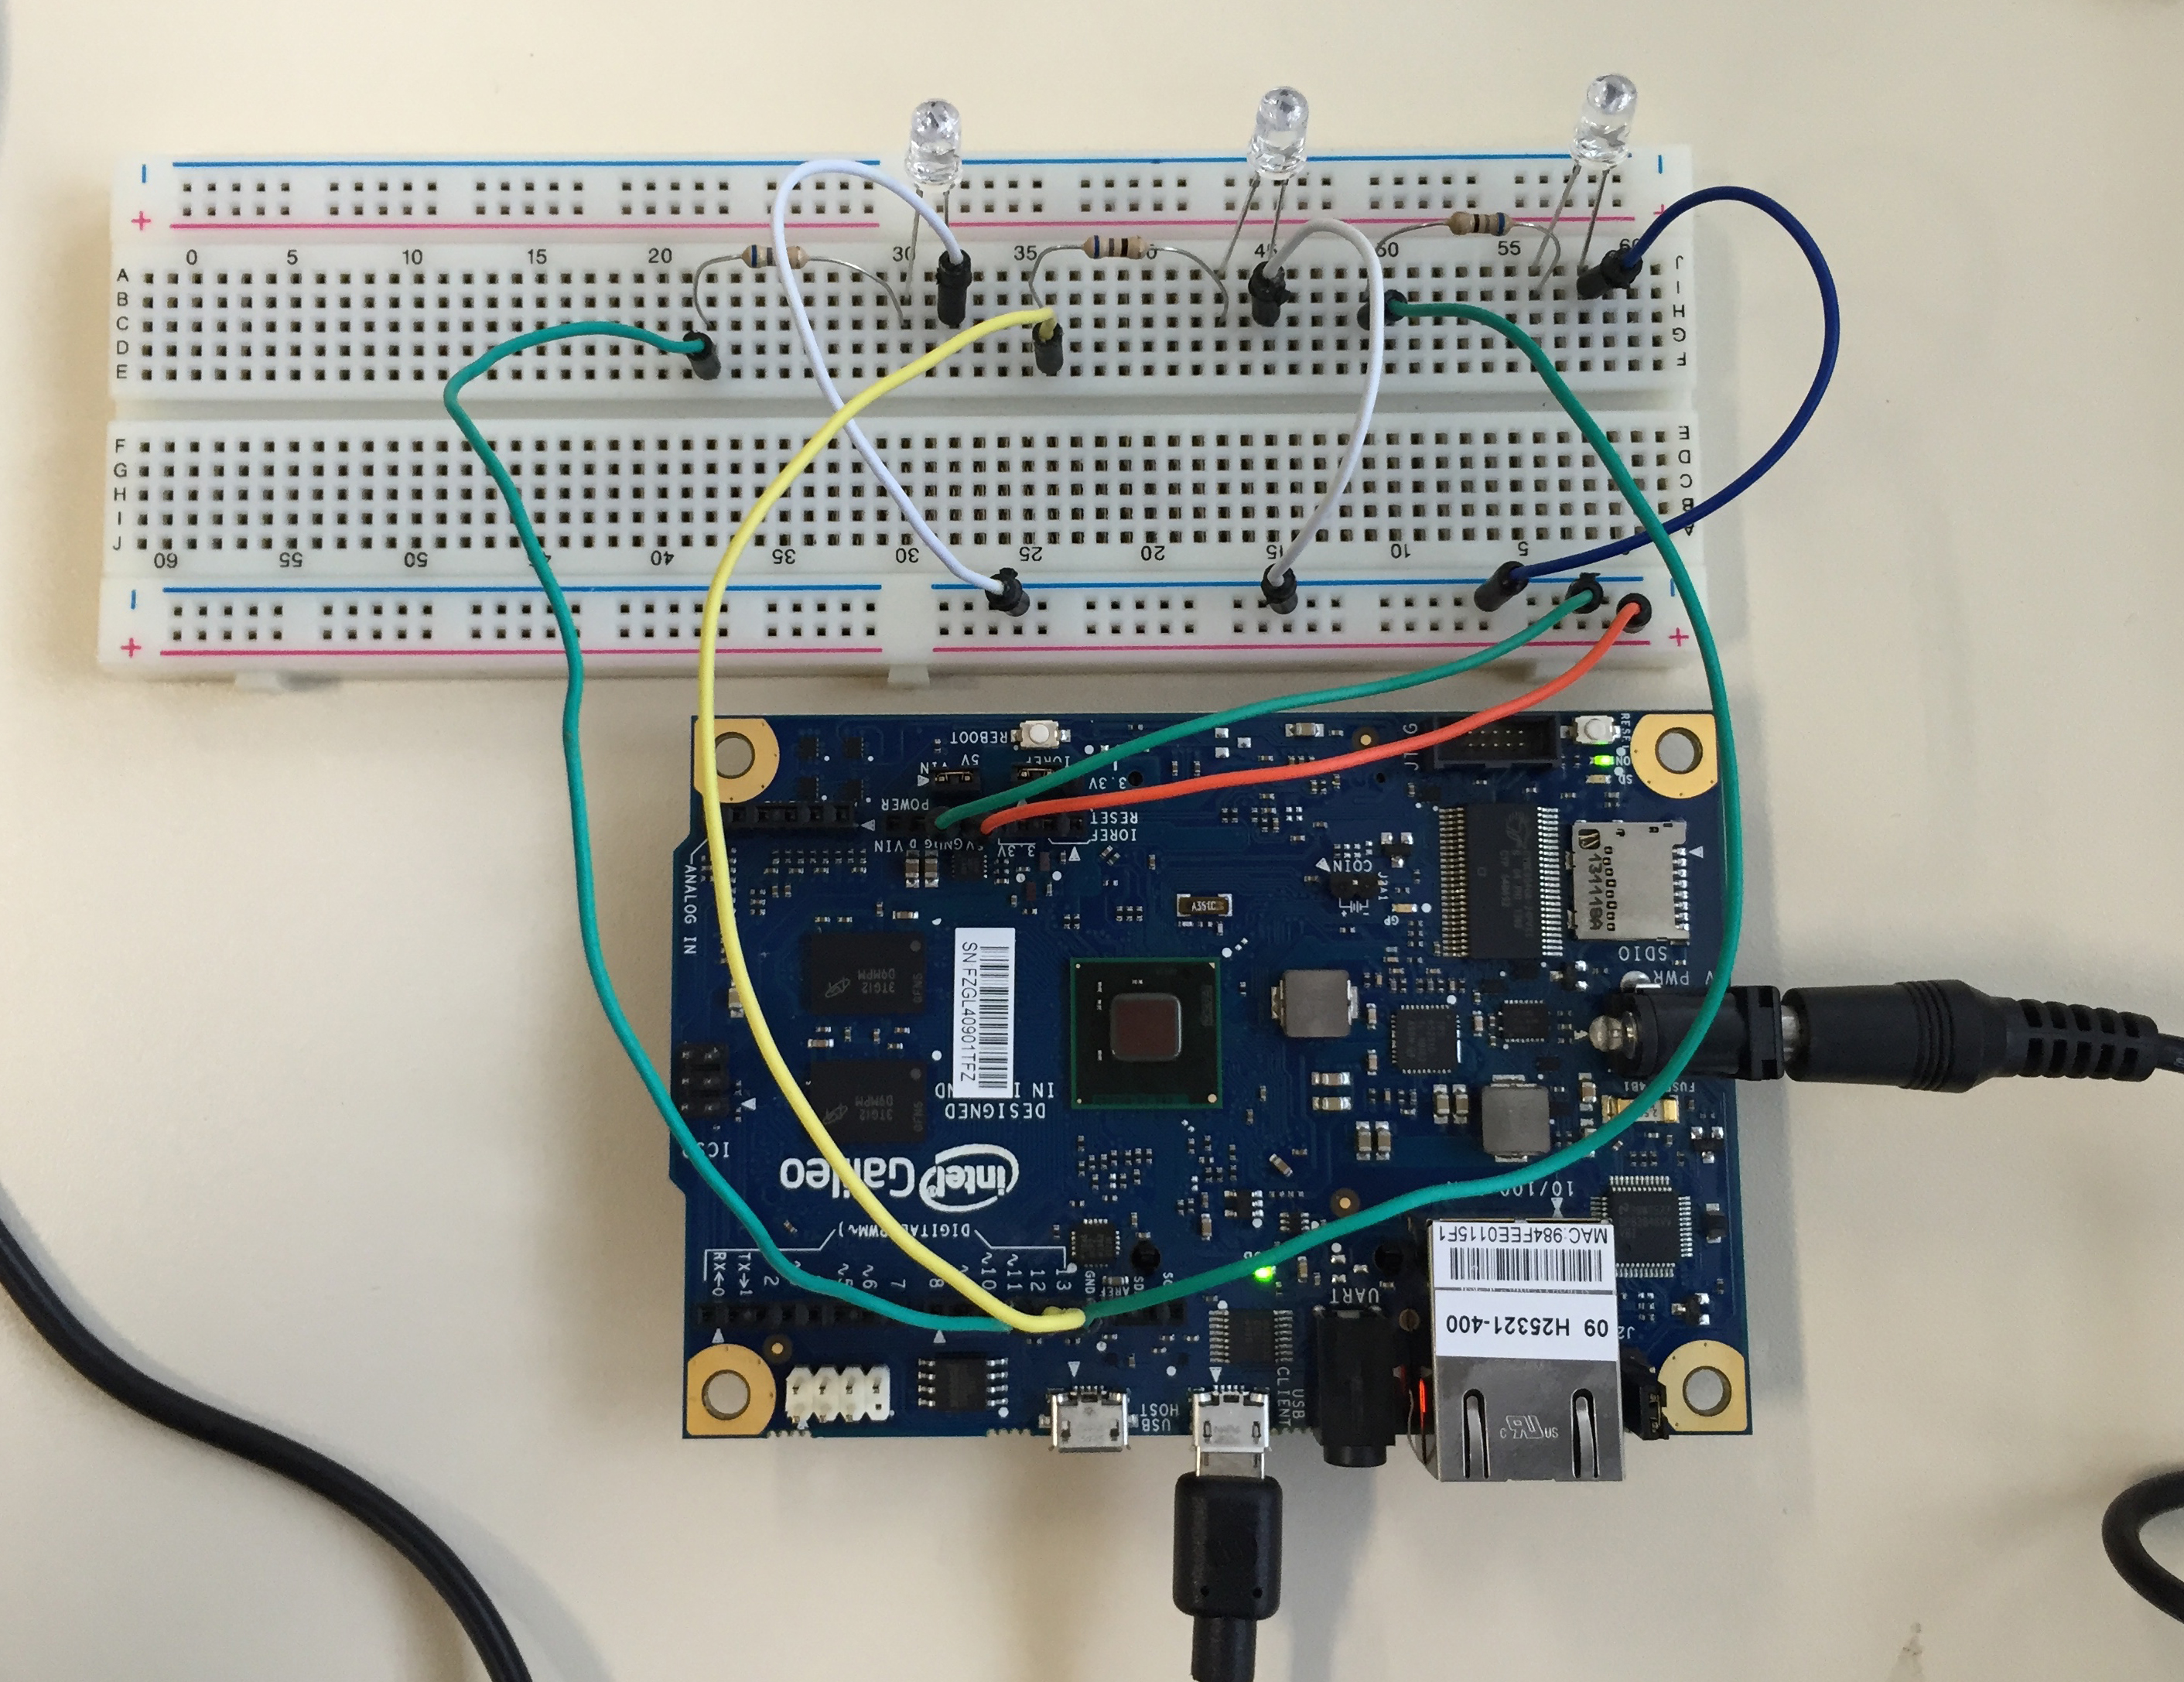
\includegraphics[scale=0.05]{chapter2/real1.jpg}
\caption{Sequência de LEDs 1}
\label{fig:3}
\end{figure}
\begin{figure}[h]
\centering
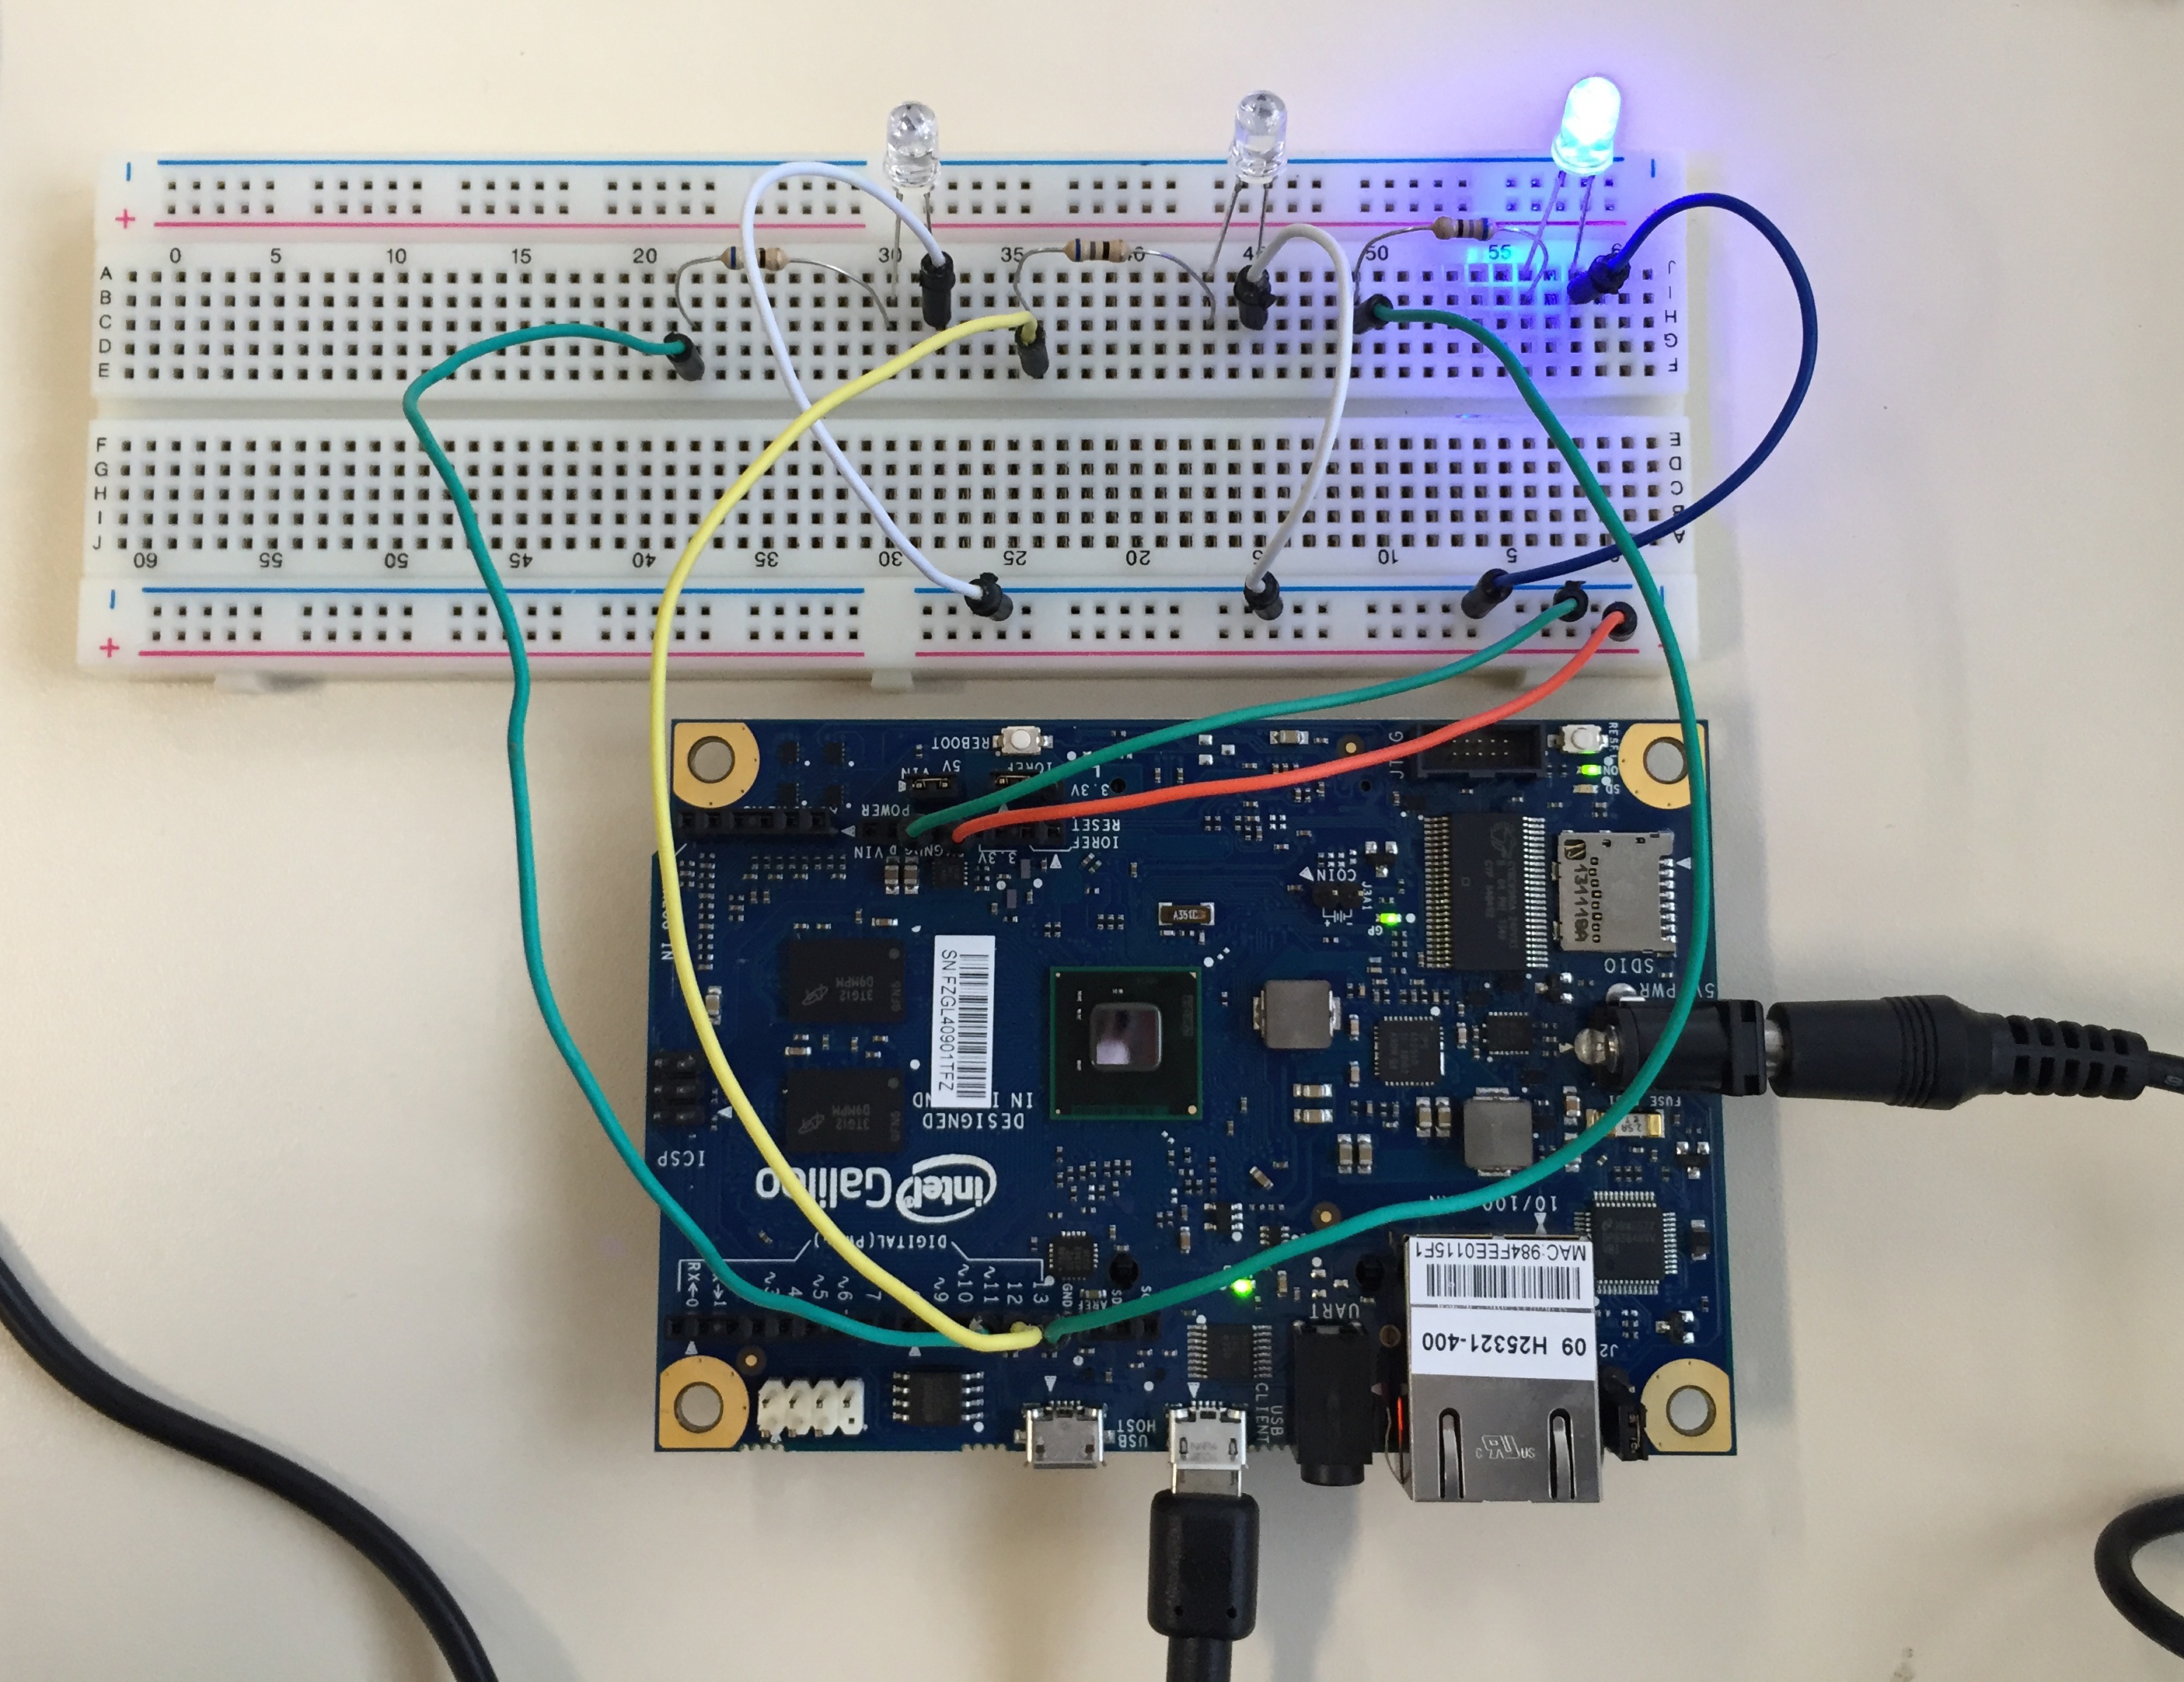
\includegraphics[scale=0.05]{chapter2/real2.jpg}
\caption{Sequência de LEDs 2}
\label{fig:4}
\end{figure}
\begin{figure}[h]
\centering
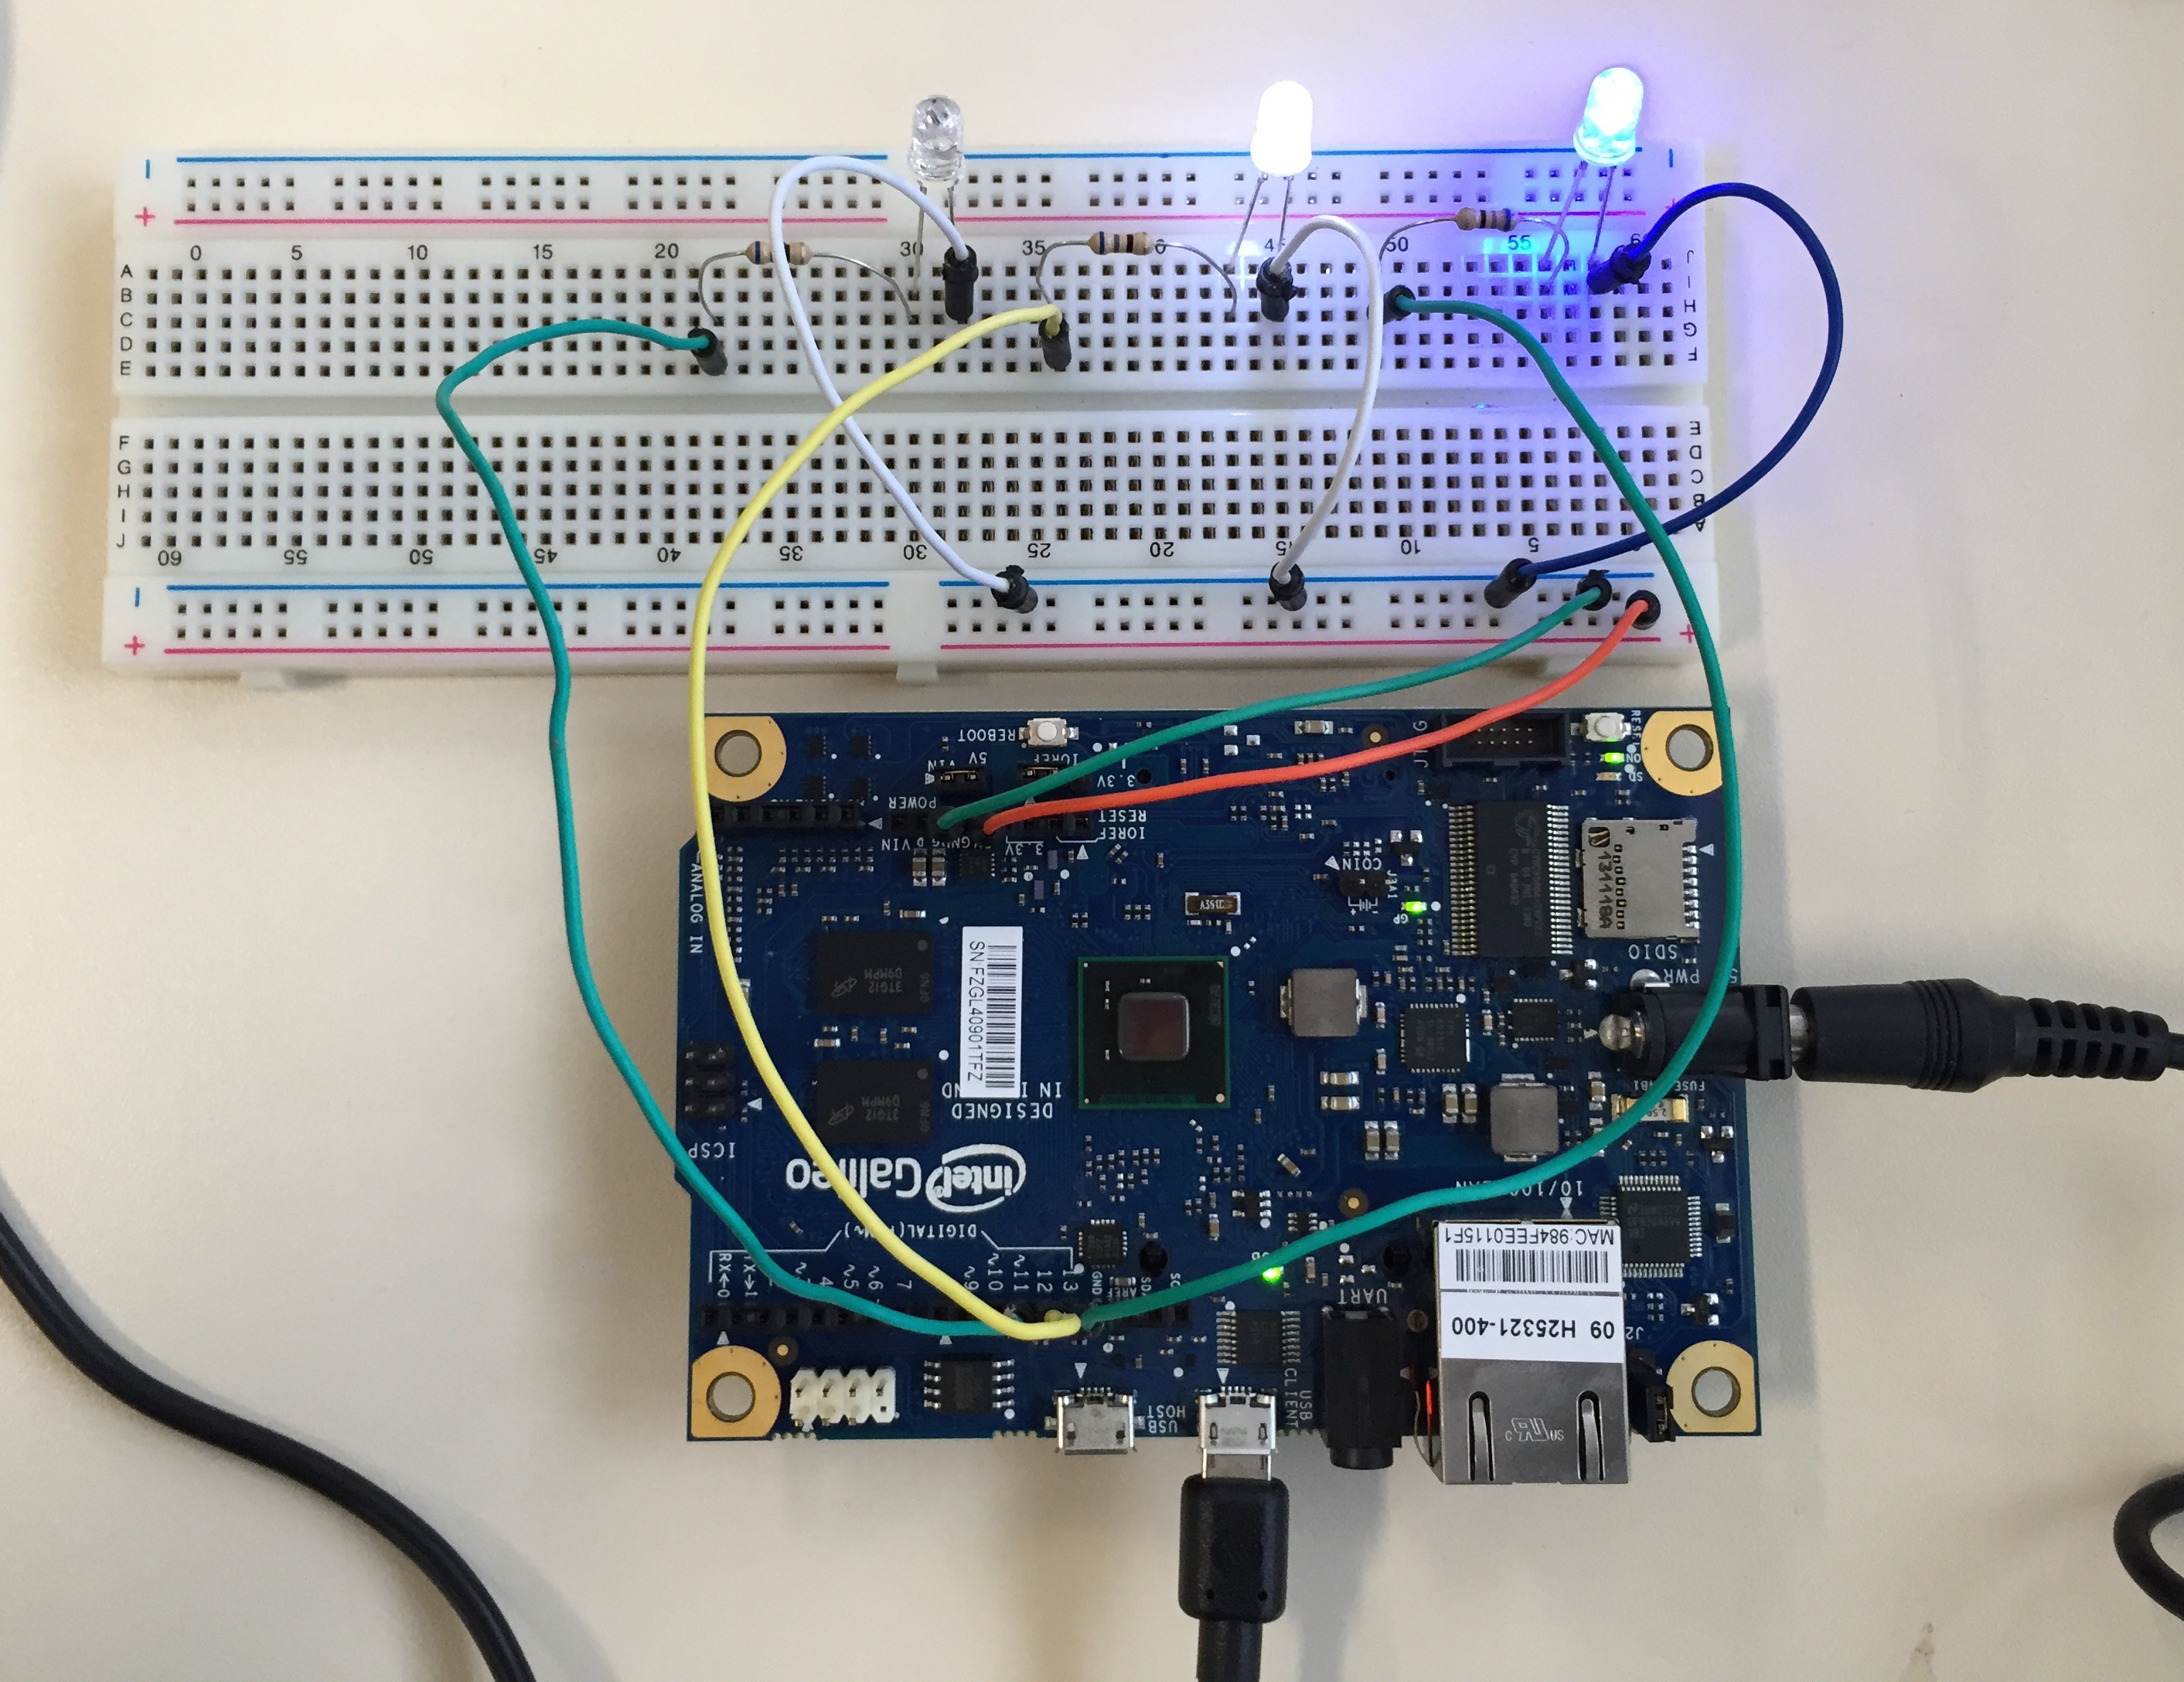
\includegraphics[scale=0.05]{chapter2/real3.jpg}
\caption{Sequência de LEDs 3}
\label{fig:5}
\end{figure}
\begin{figure}[h]
\centering
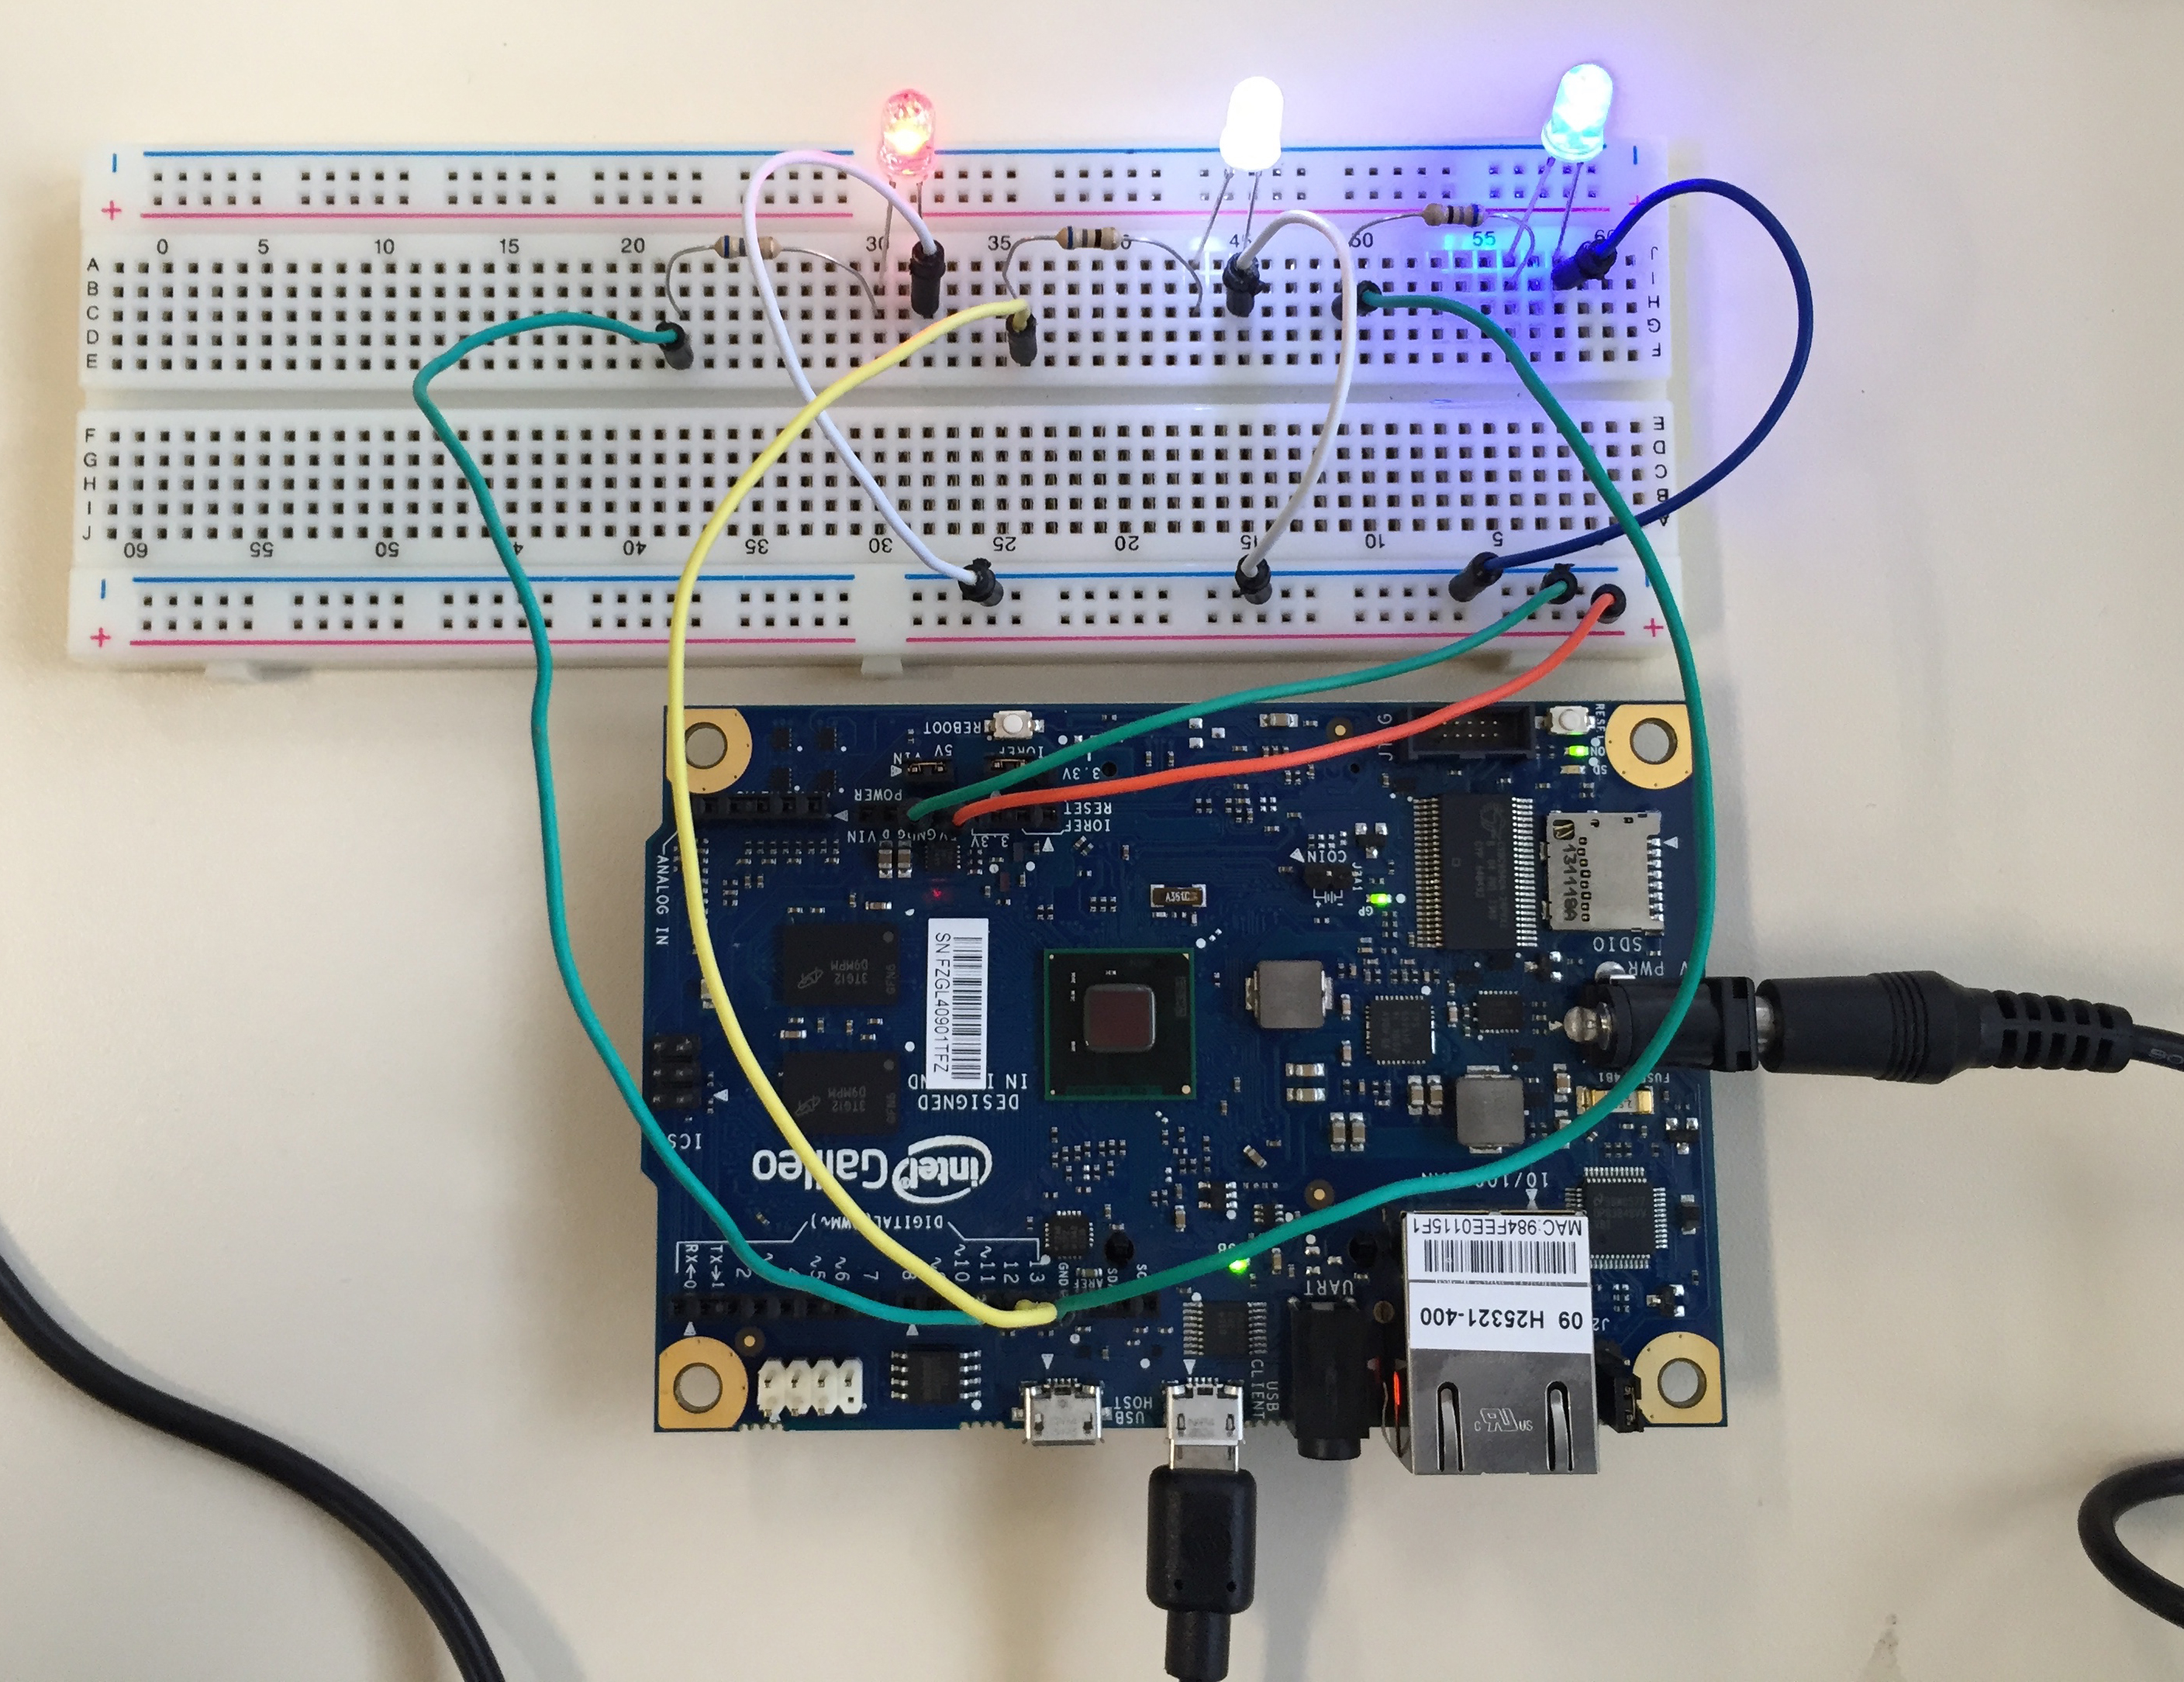
\includegraphics[scale=0.05]{chapter2/real.jpg}
\caption{Sequência de LEDs 4}
\label{fig:6}
\end{figure}
